% ============================================================
% Session 02 – Tensors in PyTorch
% Deep Learning Course – IIIT Dharwad
% Prof. S R M Prasanna & Dr. Sunil Saumya
% November 20, 2025
% ============================================================

\documentclass[12pt,a4paper]{article}
\usepackage{amsmath,amsthm,amssymb,mathtools}
\usepackage{tikz}
\usetikzlibrary{arrows.meta,positioning,shapes.geometric,calc,fit,backgrounds}
\usepackage{graphicx}
\usepackage{booktabs,tabularx,multirow}
\usepackage[ruled,vlined,linesnumbered]{algorithm2e}
\usepackage[most]{tcolorbox}
\usepackage{hyperref}
\usepackage[capitalize,noabbrev]{cleveref}
\usepackage[margin=1in]{geometry}
\usepackage{fancyhdr}
\usepackage{enumitem}
\usepackage{xcolor}
\usepackage{listings}

% ------------------------------------------------------------------
% Colour definitions
% ------------------------------------------------------------------
\definecolor{codeblue}{RGB}{0,90,160}
\definecolor{codegray}{RGB}{245,245,245}
\definecolor{keywordcolor}{RGB}{0,100,180}
\definecolor{stringcolor}{RGB}{180,0,0}
\definecolor{commentcolor}{RGB}{80,130,80}

% ------------------------------------------------------------------
% Listings style for Python
% ------------------------------------------------------------------
\lstdefinestyle{pythonstyle}{
  backgroundcolor=\color{codegray},
  basicstyle=\ttfamily\small,
  keywordstyle=\color{keywordcolor}\bfseries,
  stringstyle=\color{stringcolor},
  commentstyle=\color{commentcolor}\itshape,
  language=Python,
  breaklines=true,
  frame=single,
  framerule=0.4pt,
  rulecolor=\color{gray!60},
  showstringspaces=false,
  tabsize=4,
  numbers=left,
  numberstyle=\tiny\color{gray},
  numbersep=6pt,
}
\lstset{style=pythonstyle}

% ------------------------------------------------------------------
% tcolorbox environments
% ------------------------------------------------------------------
\newtcolorbox{keyinsight}[1][]{colback=blue!5!white,colframe=blue!75!black,fonttitle=\bfseries,title=Key Insight,#1}
\newtcolorbox{example}[1][]{colback=green!5!white,colframe=green!75!black,fonttitle=\bfseries,title=Example,#1}
\newtcolorbox{warningbox}[1][]{colback=red!5!white,colframe=red!75!black,fonttitle=\bfseries,title=Warning,#1}

% ------------------------------------------------------------------
% amsthm environments
% ------------------------------------------------------------------
\newtheorem{theorem}{Theorem}[section]
\newtheorem{lemma}[theorem]{Lemma}
\newtheorem{definition}{Definition}[section]
\newtheorem{remark}{Remark}[section]

% ------------------------------------------------------------------
% Header / footer
% ------------------------------------------------------------------
\pagestyle{fancy}
\fancyhf{}
\lhead{\textsc{Deep Learning} -- Session 02}
\rhead{Tensors in PyTorch}
\cfoot{\thepage}
\renewcommand{\headrulewidth}{0.4pt}

% ------------------------------------------------------------------
% Hyperref setup
% ------------------------------------------------------------------
\hypersetup{
  colorlinks=true,
  linkcolor=codeblue,
  urlcolor=codeblue,
  citecolor=codeblue,
  pdftitle={Session 02 -- Tensors in PyTorch},
  pdfauthor={IIIT Dharwad Deep Learning Course},
}

% ------------------------------------------------------------------
% Convenience macros
% ------------------------------------------------------------------
\newcommand{\tbf}[1]{\textbf{#1}}
\newcommand{\tit}[1]{\textit{#1}}
\newcommand{\ttt}[1]{\texttt{#1}}

% ==================================================================
\begin{document}
% ==================================================================

% ------------------------------------------------------------------
% Title page
% ------------------------------------------------------------------
\begin{titlepage}
  \centering
  \vspace*{2cm}
  {\LARGE\bfseries Deep Learning Course\\[0.4em]
   \large Indian Institute of Information Technology Dharwad\par}
  \vspace{1.5cm}
  \rule{\linewidth}{0.5pt}\\[0.6em]
  {\Huge\bfseries Session 02\\[0.3em]
   \LARGE Tensors in PyTorch\par}
  \rule{\linewidth}{0.5pt}\\[1.2cm]

  \begin{tabular}{rl}
    \tbf{Instructors:}  & Prof.\ S R M Prasanna \& Dr.\ Sunil Saumya \\[4pt]
    \tbf{Department:}   & Data Science \& Artificial Intelligence \\[4pt]
    \tbf{Institute:}    & IIIT Dharwad \\[4pt]
    \tbf{Date:}         & November 20, 2025 \\[4pt]
    \tbf{Slide Deck:}   & \texttt{02-PyTorchDL-Tensor} (17 slides) \\[4pt]
    \tbf{Notebook:}     & \texttt{TensorBasics.ipynb} \\[4pt]
    \tbf{Duration:}     & 1 hour 44 minutes \\[4pt]
    \tbf{Video:}        & \url{https://vimeo.com/1139558263} \\
  \end{tabular}

  \vfill
  {\large\itshape ``Tensors are the fundamental data structure of deep learning.
   Master them and you master the language of neural networks.''\par}
  \vspace{1cm}
\end{titlepage}

% ------------------------------------------------------------------
% Table of contents
% ------------------------------------------------------------------
\tableofcontents
\newpage

% ==================================================================
\section{Introduction}
\label{sec:intro}
% ==================================================================

Session~02 of the Deep Learning course at IIIT Dharwad is a hands-on
laboratory session dedicated to \tbf{PyTorch tensors}. The session is
structured as a live Google Colab coding walkthrough using the notebook
\ttt{TensorBasics.ipynb}, supported by the 17-slide deck
\ttt{02-PyTorchDL-Tensor}.

The instructors began with a brief recap of Session~01, which covered the
course plan, a high-level overview of machine learning and deep learning, and
the reasons for choosing PyTorch over TensorFlow. The key motivation for this
session is captured in the course philosophy:

\begin{quote}
  \itshape ``This course will be 50\% theory (mathematics and conceptual
  understanding) and 50\% practice (coding), because that is what will help you
  immediately in your projects and workplace.''
  \upshape \quad --- Dr.\ Sunil Saumya (00:11:55)
\end{quote}

The session covers the following major topics in sequence:
\begin{enumerate}[label=\arabic*.]
  \item Why tensors? GPU support, autograd, and the computation graph.
  \item Tensor dimensions: scalars, vectors, matrices, and higher-order tensors.
  \item Tensor creation functions: \ttt{torch.tensor}, \ttt{torch.zeros},
        \ttt{torch.ones}, \ttt{torch.randn}, \ttt{torch.arange},
        \ttt{torch.linspace}, \ttt{torch.eye}, \ttt{torch.full}.
  \item Tensor shapes and data types (\ttt{dtype}).
  \item Mathematical operations: unary, element-wise, reduction.
  \item Matrix multiplication and the neural network forward pass
        $\mathbf{Y} = \mathbf{W}\mathbf{X} + \mathbf{B}$.
\end{enumerate}

% ==================================================================
\section{Background and Prerequisites}
\label{sec:background}
% ==================================================================

\subsection{What is a Tensor?}

\begin{definition}[Tensor]
\label{def:tensor}
A \tbf{tensor} is a multi-dimensional array of numerical values. It generalises
the notions of scalars (0-D), vectors (1-D), and matrices (2-D) to an arbitrary
number of dimensions. In the context of PyTorch, tensors additionally support
GPU-accelerated computation and automatic differentiation.
\end{definition}

Tensors are structurally similar to NumPy \ttt{ndarray} objects but differ in
two critical respects:

\begin{itemize}[leftmargin=*]
  \item \tbf{GPU compatibility.} Tensors can be allocated on CUDA-enabled
        GPUs, enabling massive parallelism. The CUDA check in the notebook
        confirmed \texttt{torch.cuda.is\_available() = True} with PyTorch
        version \ttt{2.9.0+cu126}.
  \item \tbf{Automatic differentiation (autograd).} PyTorch tracks operations
        on tensors in a dynamic computation graph, enabling automatic
        gradient computation via backpropagation.
\end{itemize}

\subsection{Tensor Dimensions}

\Cref{tab:tensor-dims} summarises the tensor hierarchy by dimensionality and
provides deep learning examples for each rank.

\begin{table}[ht]
  \centering
  \caption{Tensor ranks, shapes, and deep learning use cases.}
  \label{tab:tensor-dims}
  \begin{tabularx}{\linewidth}{c c X X}
    \toprule
    \tbf{Rank} & \tbf{Name} & \tbf{Shape example} & \tbf{Deep Learning use case} \\
    \midrule
    0 & Scalar     & \ttt{()} or \ttt{[]}    & Loss value, learning rate, single metric \\
    1 & Vector     & \ttt{[n]}               & Bias vector, 1-D feature vector \\
    2 & Matrix     & \ttt{[m, n]}            & Weight matrix, batch of vectors \\
    3 & 3-D Tensor & \ttt{[batch, seq, feat]}& Sequence data (NLP), time series \\
    4 & 4-D Tensor & \ttt{[B, C, H, W]}      & Image batches (CNNs) \\
    5 & 5-D Tensor & \ttt{[B, D, C, H, W]}   & Video data (3-D CNNs) \\
    \bottomrule
  \end{tabularx}
\end{table}

\begin{keyinsight}[title=Tensors vs.\ NumPy Arrays]
Up to 3 dimensions, tensors and NumPy arrays are visually and structurally
identical. The difference becomes apparent at dimensions 4 and above, where
tensors provide a natural and efficient representation for data such as
image batches (\ttt{[B, C, H, W]}) that would be unwieldy to reason about
in plain NumPy.
\end{keyinsight}

\subsection{PyTorch vs.\ TensorFlow}

Both PyTorch and TensorFlow use tensors as their primary data structure, but
PyTorch's dynamic computation graph (define-by-run) makes it the framework
of choice for research and this course. TensorFlow uses a static graph
(define-then-run) by default in its original design, though TensorFlow 2.x
introduced eager execution. The course uses PyTorch exclusively.

% ==================================================================
\section{Tensor Creation in PyTorch}
\label{sec:creation}
% ==================================================================

\subsection{Environment Setup}

The session opened with a GPU availability check. This should always be the
first step in a PyTorch Colab notebook to confirm that training-speed hardware
is accessible.

\begin{lstlisting}[caption={Environment setup and GPU check (V03, 00:16:00).},
                   label={lst:setup}]
import torch
print(torch.__version__)     # Output: 2.9.0+cu126

if torch.cuda.is_available():
    print("cuda is available")
else:
    print("cuda is not available")
# Output: cuda is available
\end{lstlisting}

\subsection{Primary Creation Functions}

PyTorch provides two broad classes of creation functions:
(1) \tbf{data-initialised} tensors, created from existing Python data, and
(2) \tbf{factory functions}, which generate tensors of a specified shape
filled according to some rule (zeros, ones, random, etc.).

\subsubsection{Data-Initialised Tensors}

\begin{lstlisting}[caption={Creating tensors from data (V04, 00:21:50).},
                   label={lst:from-data}]
# From a Python nested list -- preserves dtype
a = torch.tensor([[1, 2, 3],
                  [4, 5, 6]])
# tensor([[1, 2, 3],
#         [4, 5, 6]])

# Uninitialized -- raw memory, values are garbage
b = torch.empty(2, 3)
# tensor([[1.5163e-19,  6.8316e+22,  7.1235e+28],
#         [4.6116e-24,  1.2323e+25,  7.7783e+31]])
\end{lstlisting}

\begin{warningbox}
\ttt{torch.empty()} allocates raw memory \tbf{without initialisation}.
The values returned are whatever bytes happened to be in that memory
location --- they are not zero. Only use \ttt{torch.empty} when you
plan to immediately overwrite the tensor contents.
\end{warningbox}

\subsubsection{Factory Functions: Zeros, Ones, and Random}

\begin{lstlisting}[caption={Factory functions (V05, 00:25:24).},
                   label={lst:factory}]
# All zeros
torch.zeros(2, 3)
# tensor([[0., 0., 0.],
#         [0., 0., 0.]])

# All ones
e = torch.ones(2, 3)
# tensor([[1., 1., 1.],
#         [1., 1., 1.]])

# Random normal: mean=0, std=1
e = torch.randn(2, 3)
# tensor([[ 0.0856,  0.2067,  0.6007],
#         [ 0.4394,  0.7040,  0.9578]])
\end{lstlisting}

\begin{keyinsight}[title=Weight Initialisation with \ttt{torch.randn}]
Neural network weights are almost always initialised from a random normal
distribution $\mathcal{N}(0, 1)$ using \ttt{torch.randn()}. Proper
initialisation is critical: weights that are too large cause exploding
gradients; weights that are too small cause vanishing gradients.
\end{keyinsight}

\subsubsection{Reproducibility: \ttt{torch.manual\_seed}}

\begin{lstlisting}[caption={Random seed for reproducibility (V06, 00:30:04).},
                   label={lst:seed}]
# Without seed -- different values on every run
e = torch.randn(2, 3)
# tensor([[ 0.2793,  0.2515, -0.0420],
#         [-0.3960,  0.3256,  0.9385]])

# With seed -- identical values every run
torch.manual_seed(10)
e = torch.randn(2, 3)
# tensor([[ 0.3374,  0.6029,  0.3133],
#         [-0.4156,  0.3219,  0.4119]])
\end{lstlisting}

\begin{keyinsight}[title=Why Seeds Matter]
Setting \ttt{torch.manual\_seed(n)} before any random operation ensures
that the pseudo-random number generator (PRNG) starts from the same state,
producing the same sequence of values on every run. This is essential for
\tbf{reproducible experiments}: two researchers running the same notebook
with the same seed will obtain identical results, making debugging and
scientific comparison reliable.
\end{keyinsight}

\subsubsection{Sequential and Structured Tensors}

\begin{lstlisting}[caption={\ttt{arange}, \ttt{linspace}, \ttt{eye}, \ttt{full}
                   (V07--V08, 00:33:05--00:35:05).},
                   label={lst:structured}]
# torch.arange -- like Python range(), creates integer sequence
torch.arange(0, 10)
# tensor([0, 1, 2, 3, 4, 5, 6, 7, 8, 9])

# torch.linspace -- N evenly spaced points between a and b
torch.linspace(0, 1, 5)
# tensor([0.0000, 0.2500, 0.5000, 0.7500, 1.0000])

# torch.eye -- identity matrix
torch.eye(3)
# tensor([[1., 0., 0.],
#         [0., 1., 0.],
#         [0., 0., 1.]])

# torch.full -- fill with constant value
torch.full((2, 3), 10)
# tensor([[10., 10., 10.],
#         [10., 10., 10.]])
\end{lstlisting}

\begin{example}[title=\ttt{arange} vs.\ \ttt{linspace}]
\begin{itemize}[leftmargin=*]
  \item \ttt{torch.arange(start, stop, step)} takes a \tbf{step size}. The
        exact number of output elements depends on the range and step.
  \item \ttt{torch.linspace(start, stop, n)} takes a \tbf{count}. You always
        get exactly $n$ evenly spaced values from \ttt{start} to \ttt{stop}
        (inclusive).
\end{itemize}
Use \ttt{linspace} when you need a precise number of sample points, e.g.\
when creating a grid for function plotting or interpolation.
\end{example}

% ------------------------------------------------------------------
% TikZ diagram 1: Tensor creation function tree
% ------------------------------------------------------------------
\subsection{Creation Function Overview}

\Cref{fig:creation-tree} provides a visual overview of the PyTorch tensor
creation functions covered in this session.

\begin{figure}[ht]
  \centering
  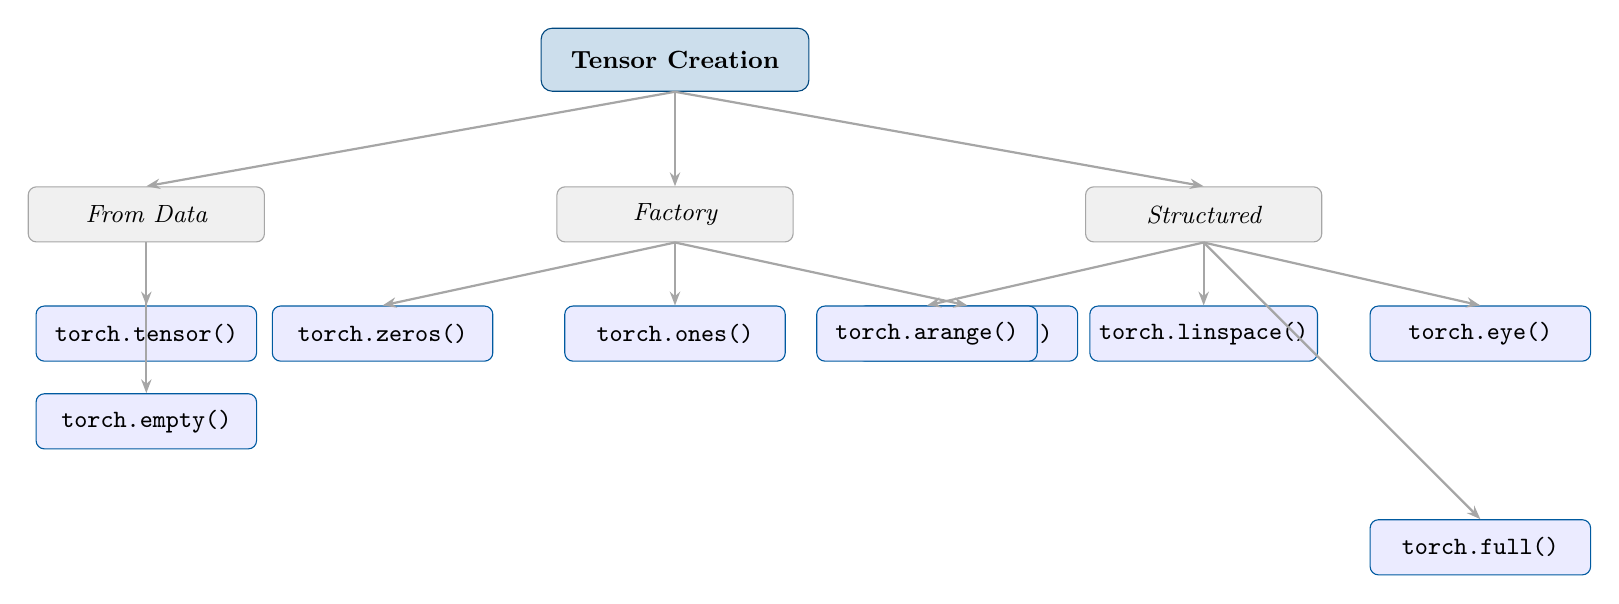
\begin{tikzpicture}[
      node distance=1.2cm and 2.2cm,
      every node/.style={font=\small},
      box/.style={rectangle, rounded corners=3pt, draw=codeblue,
                  fill=blue!8, minimum width=2.8cm, minimum height=0.7cm,
                  align=center},
      root/.style={rectangle, rounded corners=4pt, draw=codeblue!80!black,
                   fill=codeblue!20, minimum width=3.4cm, minimum height=0.8cm,
                   align=center, font=\small\bfseries},
      catbox/.style={rectangle, rounded corners=3pt, draw=gray!70,
                     fill=gray!12, minimum width=3cm, minimum height=0.7cm,
                     align=center, font=\small\itshape},
      arr/.style={-{Stealth[length=5pt]}, gray!70, thick},
    ]
    % Root
    \node[root] (root) {Tensor Creation};

    % Category nodes
    \node[catbox, below left=1.2cm and 3.5cm of root]  (fromdata) {From Data};
    \node[catbox, below=1.2cm of root]                  (factory)  {Factory};
    \node[catbox, below right=1.2cm and 3.5cm of root] (structured){Structured};

    % From-data children
    \node[box, below=0.8cm of fromdata] (tensor) {\ttt{torch.tensor()}};
    \node[box, below=0.4cm of tensor]   (empty)  {\ttt{torch.empty()}};

    % Factory children
    \node[box, below left=0.8cm and 0.8cm of factory]  (zeros) {\ttt{torch.zeros()}};
    \node[box, below=0.8cm of factory]                  (ones)  {\ttt{torch.ones()}};
    \node[box, below right=0.8cm and 0.8cm of factory] (randn) {\ttt{torch.randn()}};

    % Structured children
    \node[box, below left=0.8cm and 0.6cm of structured]  (arange)   {\ttt{torch.arange()}};
    \node[box, below=0.8cm of structured]                  (linspace) {\ttt{torch.linspace()}};
    \node[box, below right=0.8cm and 0.6cm of structured] (eye)      {\ttt{torch.eye()}};
    \node[box, below=2.0cm of eye]                         (full)     {\ttt{torch.full()}};

    % Arrows root -> categories
    \draw[arr] (root.south) -- (fromdata.north);
    \draw[arr] (root.south) -- (factory.north);
    \draw[arr] (root.south) -- (structured.north);

    % Arrows fromdata
    \draw[arr] (fromdata.south) -- (tensor.north);
    \draw[arr] (fromdata.south) -- (empty.north);

    % Arrows factory
    \draw[arr] (factory.south) -- (zeros.north);
    \draw[arr] (factory.south) -- (ones.north);
    \draw[arr] (factory.south) -- (randn.north);

    % Arrows structured
    \draw[arr] (structured.south) -- (arange.north);
    \draw[arr] (structured.south) -- (linspace.north);
    \draw[arr] (structured.south) -- (eye.north);
    \draw[arr] (structured.south) -- (full.north);
  \end{tikzpicture}
  \caption{PyTorch tensor creation functions covered in Session~02,
           organised by category.}
  \label{fig:creation-tree}
\end{figure}

% ==================================================================
\section{Tensor Shapes and Data Types}
\label{sec:shapes-dtypes}
% ==================================================================

\subsection{Shape Manipulation}
\label{subsec:shapes}

Every tensor has a \tbf{shape} attribute (\ttt{x.shape}) that returns a
\ttt{torch.Size} object --- essentially a tuple of dimension sizes.

\begin{lstlisting}[caption={Shape inspection and reshape (V09, 00:37:35).},
                   label={lst:shapes}]
x = torch.tensor([[1, 2, 3],
                  [4, 5, 6]])      # shape: (2, 3)
print(x.shape)                    # torch.Size([2, 3])

# Reshape: same data, different view
x.reshape(3, 2)
# tensor([[1, 2],
#         [3, 4],
#         [5, 6]])

# 3D tensor
torch.full((2, 3, 10), 10).shape  # torch.Size([2, 3, 10])
\end{lstlisting}

\begin{remark}
\label{rem:reshape}
\ttt{reshape} does not copy data when the new shape is compatible with the
memory layout of the original tensor; it returns a \tbf{view}. When a copy
is required (e.g.\ for non-contiguous tensors), use \ttt{.contiguous()}
followed by \ttt{.reshape()}, or use \ttt{.view()}.
\end{remark}

\subsection{Data Types (\ttt{dtype})}
\label{subsec:dtypes}

Each PyTorch tensor has a fixed numerical precision encoded in its \ttt{dtype}
attribute. \Cref{tab:dtypes} summarises the most commonly used types.

\begin{table}[ht]
  \centering
  \caption{Common PyTorch \ttt{dtype} values and their deep learning roles.}
  \label{tab:dtypes}
  \begin{tabular}{llll}
    \toprule
    \tbf{\ttt{dtype}} & \tbf{Bits} & \tbf{Range / Precision} & \tbf{Use Case} \\
    \midrule
    \ttt{torch.int64}   & 64 & Integer, large range    & Indices, integer ops \\
    \ttt{torch.float32} & 32 & $\sim$7 decimal digits  & Standard NN weights \& activations \\
    \ttt{torch.float64} & 64 & $\sim$15 decimal digits & High-precision (slower on GPU) \\
    \ttt{torch.float16} & 16 & $\sim$3 decimal digits  & Quantisation, memory reduction \\
    \ttt{torch.int8}    &  8 & $-128$ to $127$         & Extreme quantisation (LLM inference) \\
    \bottomrule
  \end{tabular}
\end{table}

\begin{lstlisting}[caption={dtype inspection and type casting (V10, 00:39:49).},
                   label={lst:dtype}]
x = torch.tensor([[1, 2, 3], [4, 5, 6]])
x.dtype     # torch.int64  (integers inferred)

y = torch.tensor([[1.0, 2.0, 3.0], [5.0, 6.0, 7.0]])
y.dtype     # torch.float32 (floats inferred)

# Explicit type casting
x.float()   # converts to torch.float32
x.double()  # converts to torch.float64
x.half()    # converts to torch.float16
\end{lstlisting}

\begin{keyinsight}[title=Quantisation and Large Language Models]
Large language models (LLMs) typically use \ttt{float16} (\ttt{fp16}) or
even \ttt{int8} precision to reduce GPU memory footprint during inference.
A model that requires 32~GB in \ttt{float32} requires only 16~GB in
\ttt{float16} and 8~GB in \ttt{int8}. This precision--efficiency trade-off
is a central technique in deploying modern deep learning systems.
\end{keyinsight}

% ------------------------------------------------------------------
% TikZ diagram 2: dtype precision ladder
% ------------------------------------------------------------------
\begin{figure}[ht]
  \centering
  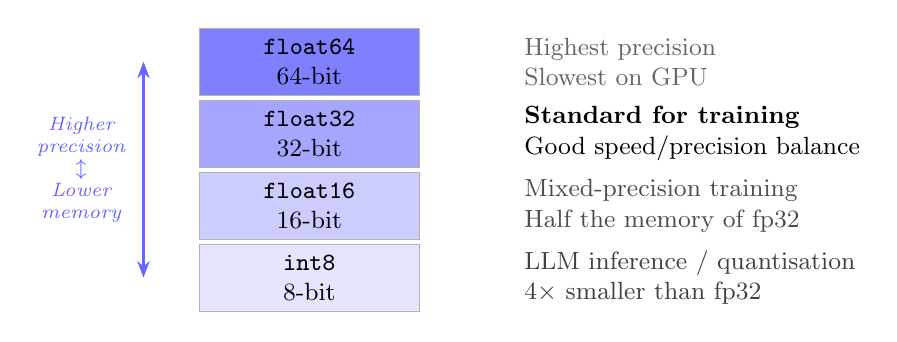
\begin{tikzpicture}[
      node distance=0.0cm,
      every node/.style={font=\small},
      dblock/.style={rectangle, draw=gray!60, fill=blue!#1, minimum width=2.8cm,
                     minimum height=0.85cm, align=center},
    ]
    % Stack of dtype blocks (left column: label; right column: bits)
    \node[dblock=50] (fp64) at (0,0)     {\ttt{float64} \\ 64-bit};
    \node[dblock=35, below=0.05cm of fp64] (fp32) {\ttt{float32} \\ 32-bit};
    \node[dblock=20, below=0.05cm of fp32] (fp16) {\ttt{float16} \\ 16-bit};
    \node[dblock=10, below=0.05cm of fp16] (int8) {\ttt{int8} \\ 8-bit};

    % Annotations on the right
    \node[right=1.2cm of fp64, align=left, text=gray!80!black] (ann64)
          {Highest precision\\ Slowest on GPU};
    \node[right=1.2cm of fp32, align=left] (ann32)
          {\textbf{Standard for training}\\ Good speed/precision balance};
    \node[right=1.2cm of fp16, align=left, text=gray!60!black] (ann16)
          {Mixed-precision training\\ Half the memory of fp32};
    \node[right=1.2cm of int8, align=left, text=gray!50!black] (ann8)
          {LLM inference / quantisation\\ 4$\times$ smaller than fp32};

    % Double arrow on left indicating precision axis
    \draw[{Stealth[length=6pt]}-{Stealth[length=6pt]}, thick, blue!60]
      ([xshift=-0.7cm]fp64.west) -- ([xshift=-0.7cm]int8.west)
      node[midway, left=0.1cm, align=center, font=\scriptsize\itshape]
           {Higher \\ precision \\ $\updownarrow$ \\ Lower \\ memory};
  \end{tikzpicture}
  \caption{PyTorch floating-point \ttt{dtype} hierarchy: precision decreases and
           memory efficiency increases from top to bottom.}
  \label{fig:dtype-ladder}
\end{figure}

% ==================================================================
\section{Mathematical Operations on Tensors}
\label{sec:math-ops}
% ==================================================================

\subsection{Unary Operations}
\label{subsec:unary}

Unary operations act on a single tensor element-by-element.

\begin{lstlisting}[caption={Unary mathematical operations (V11, 00:45:00).},
                   label={lst:unary}]
f = torch.tensor([1., 2., 3., 5., 6., 9.])

torch.abs(f)   # tensor([1., 2., 3., 5., 6., 9.])
torch.neg(f)   # tensor([-1., -2., -3., -5., -6., -9.])
torch.log(f)   # natural logarithm: ln(x)
torch.exp(f)   # e^x

# Rounding
g = torch.tensor([1.7, 2.5, 5.6, 6.9])
torch.round(g) # tensor([2., 2., 6., 7.])  -- round to nearest even
torch.ceil(g)  # tensor([2., 3., 6., 7.])  -- round up
torch.floor(g) # tensor([1., 2., 5., 6.])  -- round down
\end{lstlisting}

The rounding functions follow IEEE 754 conventions. \ttt{torch.round} uses
\tbf{banker's rounding} (round half to even), which reduces cumulative rounding
bias in large computations.

\subsection{Element-wise Binary Operations}
\label{subsec:binary}

Binary operations between two tensors of the same shape are applied
element-by-element. \Cref{eq:elemwise} formalises this for addition.

\begin{equation}
  \label{eq:elemwise}
  (\mathbf{A} + \mathbf{B})_{ij} = a_{ij} + b_{ij}, \quad
  \forall\, i \in [1, m],\; j \in [1, n]
\end{equation}

\begin{lstlisting}[caption={Element-wise arithmetic (V12, 00:53:45).},
                   label={lst:elemwise}]
a = torch.tensor([[8, 9,  4],
                  [4, 9,  4]])

b = torch.tensor([[5, 11, 12],
                  [13, 15, 4]])

a + b   # tensor([[13, 20, 16], [17, 24,  8]])
a - b   # tensor([[-3, -2, -8], [-9, -6,  0]])  (element-wise)
a * b   # element-wise product (Hadamard product)
a / b   # element-wise division
\end{lstlisting}

\begin{example}[title=Broadcasting Rules]
If two tensors have different shapes, PyTorch attempts to \tbf{broadcast}
them. A tensor of shape \ttt{[1, n]} can be added to a tensor of shape
\ttt{[m, n]} by implicitly replicating the first tensor $m$ times. Broadcasting
follows NumPy semantics: dimensions are compared from the trailing end, and a
dimension of size~1 is expanded to match the other operand.
\end{example}

\subsection{Logarithm, Exponential, and Transpose}
\label{subsec:log-exp}

\begin{lstlisting}[caption={\ttt{torch.log}, \ttt{torch.exp}, transpose, dot
                   product (V15, 01:02:46).}, label={lst:log-exp}]
# Natural logarithm
torch.log(torch.tensor([1.0, 2.0, 3.0]))
# tensor([0.0000, 0.6931, 1.0986])

# Exponential
torch.exp(torch.tensor([0.0, 1.0, 2.0]))
# tensor([1.0000, 2.7183, 7.3891])

# Transpose: swap axes
x = torch.tensor([[1, 2, 3], [4, 5, 6]])  # shape (2, 3)
x.T   # shape (3, 2)
# tensor([[1, 4],
#         [2, 5],
#         [3, 6]])

# Dot product (1-D tensors only)
a = torch.tensor([1.0, 2.0, 3.0])
b = torch.tensor([4.0, 5.0, 6.0])
torch.dot(a, b)   # 1*4 + 2*5 + 3*6 = 32.0
\end{lstlisting}

The dot product between two 1-D tensors is:
\begin{equation}
  \label{eq:dot}
  \mathbf{a} \cdot \mathbf{b} = \sum_{i=1}^{n} a_i b_i
\end{equation}

% ==================================================================
\section{Matrix Multiplication and the Neural Network Forward Pass}
\label{sec:matmul}
% ==================================================================

\subsection{The \texorpdfstring{$\mathbf{Y} = \mathbf{W}\mathbf{X} + \mathbf{B}$}{Y = WX + B} Formula}
\label{subsec:wxb}

The most important equation in all of deep learning is the linear
transformation at the heart of every fully-connected layer:

\begin{equation}
  \label{eq:linear}
  \mathbf{Y} = \mathbf{W} \mathbf{X} + \mathbf{B}
\end{equation}

where:
\begin{align}
  \mathbf{X} &\in \mathbb{R}^{d_{\text{in}} \times N} && \text{input matrix (features $\times$ batch)} \label{eq:X}\\
  \mathbf{W} &\in \mathbb{R}^{d_{\text{out}} \times d_{\text{in}}} && \text{weight matrix} \label{eq:W}\\
  \mathbf{B} &\in \mathbb{R}^{d_{\text{out}} \times 1} && \text{bias vector (broadcast over batch)} \label{eq:B}\\
  \mathbf{Y} &\in \mathbb{R}^{d_{\text{out}} \times N} && \text{pre-activation output} \label{eq:Y}
\end{align}

\begin{keyinsight}[title=Dimensions Must Be Compatible]
For $\mathbf{W}\mathbf{X}$ to be defined, the number of columns in $\mathbf{W}$
must equal the number of rows in $\mathbf{X}$. Concretely, if
$\mathbf{W} \in \mathbb{R}^{m \times k}$ and $\mathbf{X} \in \mathbb{R}^{k \times n}$,
then $\mathbf{W}\mathbf{X} \in \mathbb{R}^{m \times n}$. The \tbf{inner
dimension $k$ must match}. This is the single most common source of shape
errors in deep learning code.
\end{keyinsight}

\subsection{Matrix Multiplication: \ttt{torch.mm}}
\label{subsec:mm}

PyTorch provides \ttt{torch.mm(A, B)} for 2-D matrix multiplication. For
batched or higher-dimensional cases, use \ttt{torch.matmul(A, B)} or the
\ttt{@} operator.

\begin{lstlisting}[caption={\ttt{torch.mm} matrix multiplication (V14, 01:00:06).},
                   label={lst:mm}]
# a has shape (3, 2); b has shape (2, 3)
a = torch.tensor([[8, 9],
                  [4, 9],
                  [4, 11]])      # shape: (3, 2)

b = torch.tensor([[56, 10, 32],
                  [30, 18,  4]]) # shape: (2, 3)

# Matrix product: (3x2) @ (2x3) = (3x3)
result = torch.mm(a, b)
# tensor([[718, 242, 292],
#         [494,  202, 164],
#         [554, 238, 172]])

# Equivalent using @ operator
result2 = a @ b
\end{lstlisting}

The matrix multiplication rule is:

\begin{equation}
  \label{eq:matmul}
  C_{ij} = \sum_{k=1}^{K} A_{ik} \cdot B_{kj},
  \quad A \in \mathbb{R}^{m \times K},\; B \in \mathbb{R}^{K \times n},\;
  C \in \mathbb{R}^{m \times n}
\end{equation}

\subsection{Visualising Matrix Multiplication}

\begin{figure}[ht]
  \centering
  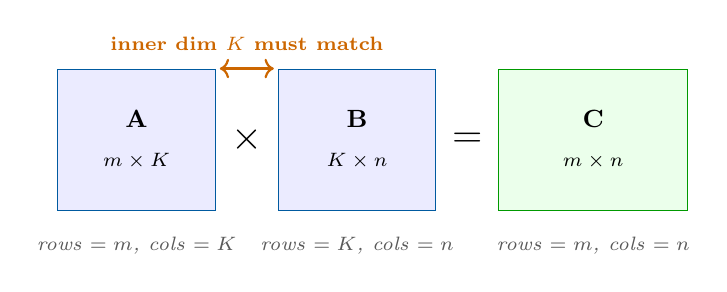
\begin{tikzpicture}[
      every node/.style={font=\small},
      mat/.style={rectangle, draw=codeblue, fill=blue!8,
                  minimum width=#1, minimum height=1.8cm, align=center},
      label_n/.style={font=\scriptsize\itshape, text=gray!70!black},
    ]
    % Matrix A
    \node[mat=2cm] (A) at (0,0) {$\mathbf{A}$\\[3pt]\scriptsize$m \times K$};
    % Times symbol
    \node at (1.4,0) {\Large$\times$};
    % Matrix B
    \node[mat=2cm] (B) at (2.8,0) {$\mathbf{B}$\\[3pt]\scriptsize$K \times n$};
    % Equals symbol
    \node at (4.2,0) {\Large$=$};
    % Matrix C
    \node[mat=2.4cm, fill=green!8, draw=green!60!black] (C) at (5.8,0)
          {$\mathbf{C}$\\[3pt]\scriptsize$m \times n$};

    % Dimension labels below
    \node[label_n, below=0.2cm of A] {rows $= m$, cols $= K$};
    \node[label_n, below=0.2cm of B] {rows $= K$, cols $= n$};
    \node[label_n, below=0.2cm of C] {rows $= m$, cols $= n$};

    % Matching inner dimension brace
    \draw[<->, thick, orange!80!black]
      ([xshift=0.05cm]A.north east) -- ([xshift=-0.05cm]B.north west)
      node[midway, above=0.1cm, font=\scriptsize\bfseries,
           text=orange!80!black] {inner dim $K$ must match};
  \end{tikzpicture}
  \caption{Schematic of matrix multiplication. The inner dimension $K$ (columns
           of $\mathbf{A}$ and rows of $\mathbf{B}$) must agree. The output
           has shape $(m \times n)$.}
  \label{fig:matmul}
\end{figure}

\subsection{Session Example: \ttt{a (3 \texttimes{} 2) @ b (2 \texttimes{} 3)}}

The notebook demonstrated the shape rule concretely:

\begin{align}
  \mathbf{a} &= \begin{pmatrix} 8 & 9 \\ 4 & 9 \\ 4 & 11 \end{pmatrix}_{3\times 2},
  &
  \mathbf{b} &= \begin{pmatrix} 56 & 10 & 32 \\ 30 & 18 & 4 \end{pmatrix}_{2\times 3}
  \label{eq:example-ab}
\end{align}

\begin{equation}
  \mathbf{c}_{11} = 8 \times 56 + 9 \times 30 = 448 + 270 = 718
  \label{eq:c11}
\end{equation}

% ------------------------------------------------------------------
% Algorithm: Forward pass of a single linear layer
% ------------------------------------------------------------------
\subsection{Algorithm: Forward Pass of a Fully-Connected Layer}
\label{subsec:algorithm}

\begin{algorithm}[H]
  \caption{Forward Pass --- Single Fully-Connected Layer}
  \label{alg:forward}
  \DontPrintSemicolon
  \KwIn{Input tensor $\mathbf{X} \in \mathbb{R}^{d_{\text{in}} \times N}$,
        weight matrix $\mathbf{W} \in \mathbb{R}^{d_{\text{out}} \times d_{\text{in}}}$,
        bias vector $\mathbf{b} \in \mathbb{R}^{d_{\text{out}}}$,
        activation function $\sigma(\cdot)$}
  \KwOut{Output activations $\mathbf{A} \in \mathbb{R}^{d_{\text{out}} \times N}$}
  \BlankLine
  \tcp{Step 1: linear transformation}
  $\mathbf{Z} \leftarrow \mathbf{W} \cdot \mathbf{X}$
  \tcp*{shape: $(d_{\text{out}} \times N)$}
  \BlankLine
  \tcp{Step 2: add bias (broadcast over batch dimension)}
  \For{$j \leftarrow 1$ \KwTo $N$}{
    $\mathbf{Z}_{:,j} \leftarrow \mathbf{Z}_{:,j} + \mathbf{b}$
  }
  \BlankLine
  \tcp{Step 3: apply non-linear activation}
  $\mathbf{A} \leftarrow \sigma(\mathbf{Z})$
  \BlankLine
  \Return $\mathbf{A}$
\end{algorithm}

In PyTorch, Steps 1 and 2 collapse to a single line:
\begin{equation}
  \label{eq:torch-linear}
  \texttt{Y = torch.mm(W, X) + b}
\end{equation}

where \ttt{b} is broadcast automatically over the batch dimension.

% ==================================================================
\section{Complete Operations Reference}
\label{sec:reference}
% ==================================================================

\Cref{tab:ops-reference} is a comprehensive reference of all tensor operations
covered in Session~02.

\begin{table}[ht]
  \centering
  \caption{Complete reference of PyTorch tensor operations covered in Session~02.}
  \label{tab:ops-reference}
  \begin{tabularx}{\linewidth}{l l X}
    \toprule
    \tbf{Operation} & \tbf{Function / Syntax} & \tbf{Notes} \\
    \midrule
    \multicolumn{3}{l}{\itshape Creation} \\
    \midrule
    From data        & \ttt{torch.tensor([...])}       & Infers \ttt{dtype} from Python data \\
    Uninitialized    & \ttt{torch.empty(m, n)}         & Raw memory --- values are garbage \\
    All zeros        & \ttt{torch.zeros(m, n)}         & Default \ttt{dtype}: \ttt{float32} \\
    All ones         & \ttt{torch.ones(m, n)}          & Default \ttt{dtype}: \ttt{float32} \\
    Random normal    & \ttt{torch.randn(m, n)}         & $\mathcal{N}(0,1)$; use for weight init \\
    Sequential       & \ttt{torch.arange(start, stop)} & Like Python \ttt{range()} \\
    Evenly spaced    & \ttt{torch.linspace(a, b, n)}   & Exactly $n$ points from $a$ to $b$ \\
    Identity         & \ttt{torch.eye(n)}              & $n \times n$ identity matrix \\
    Constant fill    & \ttt{torch.full(size, val)}     & All elements set to \ttt{val} \\
    \midrule
    \multicolumn{3}{l}{\itshape Shape \& Type} \\
    \midrule
    Shape            & \ttt{x.shape}                   & Returns \ttt{torch.Size} \\
    Reshape          & \ttt{x.reshape(m, n)}           & Returns a view if possible \\
    Transpose        & \ttt{x.T}                       & Swaps all axes (2-D: rows $\leftrightarrow$ cols) \\
    Data type        & \ttt{x.dtype}                   & e.g.\ \ttt{torch.float32} \\
    Cast to float32  & \ttt{x.float()}                 & \ttt{torch.float32} \\
    Cast to float64  & \ttt{x.double()}                & \ttt{torch.float64} \\
    Cast to float16  & \ttt{x.half()}                  & \ttt{torch.float16} \\
    \midrule
    \multicolumn{3}{l}{\itshape Unary Math} \\
    \midrule
    Absolute value   & \ttt{torch.abs(x)}              & $|x_{ij}|$ \\
    Negation         & \ttt{torch.neg(x)}              & $-x_{ij}$ \\
    Natural log      & \ttt{torch.log(x)}              & $\ln(x_{ij})$ \\
    Exponential      & \ttt{torch.exp(x)}              & $e^{x_{ij}}$ \\
    Round            & \ttt{torch.round(x)}            & Banker's rounding \\
    Ceiling          & \ttt{torch.ceil(x)}             & $\lceil x_{ij} \rceil$ \\
    Floor            & \ttt{torch.floor(x)}            & $\lfloor x_{ij} \rfloor$ \\
    \midrule
    \multicolumn{3}{l}{\itshape Binary \& Reduction} \\
    \midrule
    Element-wise add & \ttt{a + b}                     & Same shape or broadcastable \\
    Element-wise sub & \ttt{a - b}                     & \\
    Element-wise mul & \ttt{a * b}                     & Hadamard product \\
    Element-wise div & \ttt{a / b}                     & \\
    Dot product      & \ttt{torch.dot(a, b)}           & 1-D tensors only; returns scalar \\
    Matrix multiply  & \ttt{torch.mm(A, B)}            & 2-D only; inner dims must match \\
    General matmul   & \ttt{torch.matmul(A, B)} or \ttt{A @ B} & Works for batched / N-D \\
    Seed             & \ttt{torch.manual\_seed(n)}     & Set before \ttt{randn} for reproducibility \\
    \bottomrule
  \end{tabularx}
\end{table}

% ==================================================================
\section{Summary and Conclusions}
\label{sec:summary}
% ==================================================================

Session~02 provided a thorough hands-on introduction to PyTorch tensors, the
fundamental data structure underlying all deep learning computations. Starting
from environment setup and GPU verification, the session systematically built
tensor literacy through live coding in \ttt{TensorBasics.ipynb}.

\subsection*{Key Takeaways}

\begin{enumerate}[label=\arabic*., leftmargin=*]
  \item \tbf{Tensors generalise arrays.} They extend NumPy \ttt{ndarray}
        semantics to arbitrary rank, with native GPU support and automatic
        differentiation. The difference from NumPy becomes practically
        significant at rank~4 and above (e.g.\ image batches).

  \item \tbf{Eight creation functions.} The session covered
        \ttt{torch.tensor}, \ttt{torch.empty}, \ttt{torch.zeros},
        \ttt{torch.ones}, \ttt{torch.randn}, \ttt{torch.arange},
        \ttt{torch.linspace}, \ttt{torch.eye}, and \ttt{torch.full}.
        Each has a specific use case; choosing the right one leads to
        cleaner, more intentional code.

  \item \tbf{Seeds ensure reproducibility.} \ttt{torch.manual\_seed(n)}
        must be called before any random tensor creation to guarantee
        identical results across runs --- essential for scientific
        experiments.

  \item \tbf{\ttt{dtype} governs precision and memory.} The default
        \ttt{float32} balances precision and GPU speed. \ttt{float16}
        and \ttt{int8} are used in production inference to reduce memory,
        while \ttt{float64} is reserved for high-precision scientific work.

  \item \tbf{Matrix multiplication is the core of deep learning.}
        The forward pass of every fully-connected layer is
        $\mathbf{Y} = \mathbf{W}\mathbf{X} + \mathbf{B}$, computed via
        \ttt{torch.mm} (2-D) or \ttt{torch.matmul} (N-D). The inner
        dimension must match: $\mathbf{W}_{m \times K} \cdot \mathbf{X}_{K \times n}
        = \mathbf{Y}_{m \times n}$.
\end{enumerate}

\subsection*{Looking Ahead}

Session~03 will build on this foundation, introducing the PyTorch autograd
engine that enables automatic gradient computation through the same tensor
operations practised today. The $\mathbf{Y} = \mathbf{W}\mathbf{X} + \mathbf{B}$
formula will gain a backward pass, connecting tensor operations directly to
the parameter update rule of stochastic gradient descent.

\vspace{1cm}
\hrule
\vspace{0.5cm}
\begin{center}
  \small
  \textit{Session 02 -- Tensors in PyTorch} \\
  Deep Learning Course, IIIT Dharwad \\
  Prof.\ S R M Prasanna \& Dr.\ Sunil Saumya \\
  November 20, 2025
\end{center}

\end{document}
